La sesión analizada contó con un total de 70 senadores,
pertenecientes a 27 partidos políticos, distribuidos del
siguiente modo (Figura \ref{fig-distrib-senators}):

\begin{figure}[h!]
\centering
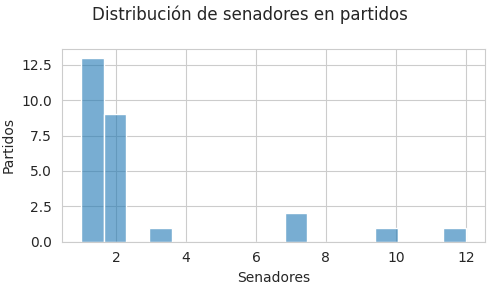
\includegraphics[scale=0.7]{../visualizations/distrib_histplot_senators_parties.png}
\caption{Distribución de senadores en partidos políticos y en provincias.}
\label{fig-distrib-senators}
\end{figure}

Aquí vemos que solo uno de los partidos (Frente de todos) cuenta con 12
senadores; también uno solo (Alianza frente para la victoria) es
representado por 10 senadores; dos partidos (Alianza cambiemos y
Juntos por el cambio) cuentan con 7 senadores, y el resto de los
partidos tienen entre 3, 2 y un senador.
En cuanto a las provincias (24 en total), todas tienen 3 senadores
exceptuando a Tucumán y a La Rioja, que tienen solo 2.

La figura \ref{fig-distrib-vote} nos muestra además que la intención
de voto no guarda una relación unívoca con los partidos a los cuales los
senadores representan. A excepción de los partidos que cuentan con un único
senador, la mayoría cuenta con senadores que votaron a favor y senadores
que votaron en contra de la ley para el acceso al aborto. Aquí también
es posible ver que un senador del Frente Justicialista se abstuvo de votar,
mientras que dos senadores, uno de Cambiemos Fuerza Cívica Riojana y uno de
Frente Unidad Justicialista San Luis, estuvieron ausentes en la votación.

\begin{figure}[h!]
\centering
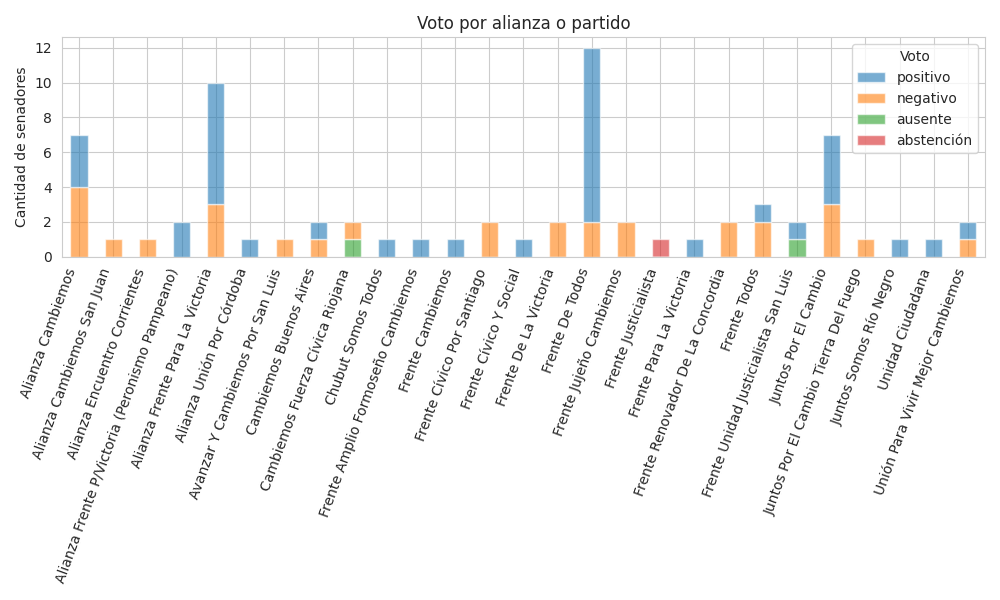
\includegraphics[scale=0.48]{../visualizations/senators_vote_by_party.png}
\caption{Distribución de votos en los distintos partidos políticos.}
\label{fig-distrib-vote}
\end{figure}

Por último, al considerar las intervenciones discursivas, observamos que
9 senadores no intervinieron en la sesión, y las intervenciones de los
restantes 61 senadores fueron resumidas en la Tabla \ref{table-tokens}, que plasma
las métricas univariadas de la cantidad de tokens totales y únicos y nos
permite observar que ambas obedecen una distribución sesgada a izquierda.

%\begin{figure}[h!]
%\centering
%\includegraphics[scale=0.6]{../visualizations/tokens_vote.png}
%\caption{Distribución de tokens emitidos por los oradores en relación a
%su intención de voto.}
%\label{fig-distrib-tokens-vote}
%\end{figure}

La Figura \ref{fig-distrib-tokens-vote}, por otro lado, nos muestra,
de forma más detallada, la distribución de los tokens emitidos según
la intención de voto de los oradores.

\begin{table}[h!]
\begin{center}
\begin{tabular}{ |c|c|c|c| }
\hline
Tokens & Media & Mediana & Desvío Estándar \\
\hline\hline
Totales & 811.65 & 636.12 & 714.79 \\
\hline
Únicos & 296.47 & 254.25 & 238.68 \\
\hline
\end{tabular}
\caption{M\'etricas univariadas de la cantidad de tokens}
\label{table-tokens}
\end{center}
\end{table}
